\documentclass[12pt,a4paper,oneside]{article}
%\documentclass[12pt,a4paper,oneside,twocolumn]{article}
\usepackage{pagestyle}
\usepackage{codestyle}

% Report hand-in date
\DTMsavedate{date}{2024-03-29}

\title{
    \Huge{Machine Learning} \\ \LARGE 
    Nature's Quest: Deep Learning Exploration of Global Plant Traits from Images and Geodata
}
\author{
Kai E. Niermann \and
Dávid Miklo \and 
Trix Taicet \and
Red Kaláb \and
Conner Dassen
}
\date{\DTMusedate{date}}
\begin{document}
\maketitle

% \lstinputlisting[firstline=10, lastline=13]{code/sample_script.py}

\begin{abstract}
    % Abstract content goes here
\end{abstract}

\section{Introduction}
% primary paragraph 
Global warming and more broadly climate change has become a major concern for the world as its effects are becoming more and more apparent \cite{WANG2023100237}. Changing weather patterns, especially towards more extreme conditions are causing plants to adapt to new environments \cite{GRAY201664}. One method of measuring said adaptation is to look at the traits, that is, properties of a plant that describe how it functions and interacts with the environment. These traits include but are not limited to of the plant height, leaf area, but also dry mass, leaf nitrogen content amongst various others. Monitoring these traits allows us to gain vital insights into how climate change impacts different ecosystems. While somewhat simple manual measurement techniques exist, at scale they are not feasible. This is where Convolutional Neural Networks (CNN) come in.  

\smallskip
Through the work demonstrated by Schiller et al \cite{schiller2021deep} we know that CNNs can be used to predict plant traits from images. The images used to train this network came from \textit{citizen science photographs} which are images taken by citizens of plants from all across the world using AI plant species identification apps (e.g. iNaturalist, Pl@ntNet). Citizen science photographs also come with location metadata, which can be used to extract ancillary geodata such as precipitation, temperature, and soil type. This geodata can optionally be combined with the images to create a CNN which can potentially learn to extract features from images in conjunction with geodata to predict plant traits.

\smallskip
For our method we wanted to compare the accuracy of a CNN trained on images alone and using a pretrained backbone (e.g. ResNet, EfficientNet, etc.) to a CNN trained on images and geodata. We hypothesize that the CNN trained on images and geodata will outperform the CNN trained on images alone. Although the geodata could potentially lead the model to learning features not necessarily helpful for accurate prediction of plant traits due to a multitiude of reasons. 


% secondary paragraph
% \section{Literature review}

\section{Method}

\subsection{Data processing}

Integral to any machine learning model is the data used to train, validate and ultimate test the model. The data used consisted of 3 main components: ancillary geodata from various sources, the main task trait means and auxillary task standard deviations, and the training images of the plants.

\smallskip 
Upon visual inspection one of the first issues we spotted was a considerable chunk (29.53\%) of missing data missing for the auxillary task standard deviations. Through some previous work on the same Kaggle we noticed that the auxillary data was a useful inclusion. We can also validate these reports with previous work applying auxillary tasks in CNNs such as the work of Lukas Libel and Marco Kroener which confirmed that the inclusion of an auxillary task with minor relevance to the main task did indeed boost performance \cite{lukaslibel} or Chen et. al. \cite{pmlr-v80-chen18a} which demonstrated that for very similar or mostly similar auxillary tasks the contribution is generally a positive one. Based on this we decided to use a simple k-nearest neighbor (kNN) imputation strategy. The rest of the data had all values present.

\smallskip
The geodata was another point of consideration in the data pre-processing phase. Looking at the individual columns we noticed that the instances had features which encoded similar information and thus where likely redundant in the training process. Since we are working with a very high dimensional feature space to get some sort of visual verification of this claim we plotted a correlation heatmap for the 3 biggest groups of the geodata, namely the datasets: soil (soil information), MODIS, and VOD.

\begin{figure}[!h]
    \centering
    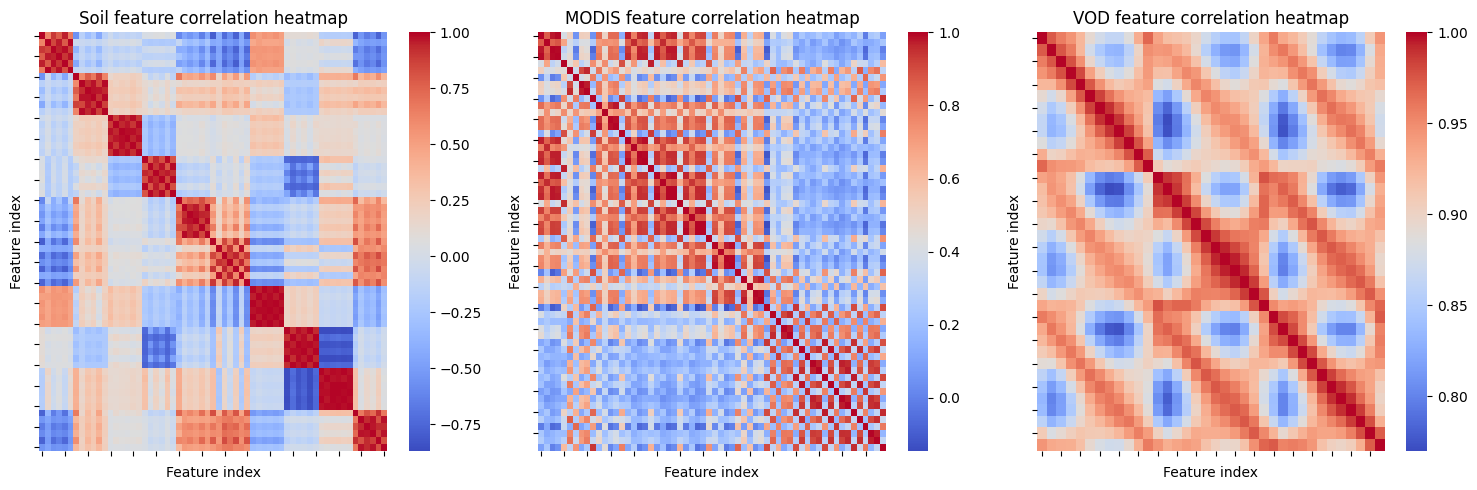
\includegraphics[width=0.9\textwidth]{assets/corr_hm.png}
    \caption{Correlation heatmap of the 3 biggest groups of geodata}
\end{figure}

Since these datasets individually can be broken down into groups of features generally talking about a similar topic we can see that the correlation within these groups is quite high. Even though previous work \cite{DBLP:journals/corr/abs-2007-00062} has demonstrated the viability of neural network models to learn from high dimensional data, removing redundant features has in numerous instances been shown to improve model performance \cite{chen2022survey}. With this in mind we decided to apply a Principal Component Analysis (PCA) to the geodata to reduce the dimensionality of the data. We specified that the number of principle components should be such that 95\% of the variance is explained.   

\subsection{Data preparation}

\subsection{Model design}

\subsection{Model evaluation}

\section{Results}

\section{Discussion}

\section{Conclusion}

\printbibliography

\end{document}